% GNUPLOT: LaTeX picture with Postscript
\begingroup
  \makeatletter
  \providecommand\color[2][]{%
    \GenericError{(gnuplot) \space\space\space\@spaces}{%
      Package color not loaded in conjunction with
      terminal option `colourtext'%
    }{See the gnuplot documentation for explanation.%
    }{Either use 'blacktext' in gnuplot or load the package
      color.sty in LaTeX.}%
    \renewcommand\color[2][]{}%
  }%
  \providecommand\includegraphics[2][]{%
    \GenericError{(gnuplot) \space\space\space\@spaces}{%
      Package graphicx or graphics not loaded%
    }{See the gnuplot documentation for explanation.%
    }{The gnuplot epslatex terminal needs graphicx.sty or graphics.sty.}%
    \renewcommand\includegraphics[2][]{}%
  }%
  \providecommand\rotatebox[2]{#2}%
  \@ifundefined{ifGPcolor}{%
    \newif\ifGPcolor
    \GPcolortrue
  }{}%
  \@ifundefined{ifGPblacktext}{%
    \newif\ifGPblacktext
    \GPblacktexttrue
  }{}%
  % define a \g@addto@macro without @ in the name:
  \let\gplgaddtomacro\g@addto@macro
  % define empty templates for all commands taking text:
  \gdef\gplbacktext{}%
  \gdef\gplfronttext{}%
  \makeatother
  \ifGPblacktext
    % no textcolor at all
    \def\colorrgb#1{}%
    \def\colorgray#1{}%
  \else
    % gray or color?
    \ifGPcolor
      \def\colorrgb#1{\color[rgb]{#1}}%
      \def\colorgray#1{\color[gray]{#1}}%
      \expandafter\def\csname LTw\endcsname{\color{white}}%
      \expandafter\def\csname LTb\endcsname{\color{black}}%
      \expandafter\def\csname LTa\endcsname{\color{black}}%
      \expandafter\def\csname LT0\endcsname{\color[rgb]{1,0,0}}%
      \expandafter\def\csname LT1\endcsname{\color[rgb]{0,1,0}}%
      \expandafter\def\csname LT2\endcsname{\color[rgb]{0,0,1}}%
      \expandafter\def\csname LT3\endcsname{\color[rgb]{1,0,1}}%
      \expandafter\def\csname LT4\endcsname{\color[rgb]{0,1,1}}%
      \expandafter\def\csname LT5\endcsname{\color[rgb]{1,1,0}}%
      \expandafter\def\csname LT6\endcsname{\color[rgb]{0,0,0}}%
      \expandafter\def\csname LT7\endcsname{\color[rgb]{1,0.3,0}}%
      \expandafter\def\csname LT8\endcsname{\color[rgb]{0.5,0.5,0.5}}%
    \else
      % gray
      \def\colorrgb#1{\color{black}}%
      \def\colorgray#1{\color[gray]{#1}}%
      \expandafter\def\csname LTw\endcsname{\color{white}}%
      \expandafter\def\csname LTb\endcsname{\color{black}}%
      \expandafter\def\csname LTa\endcsname{\color{black}}%
      \expandafter\def\csname LT0\endcsname{\color{black}}%
      \expandafter\def\csname LT1\endcsname{\color{black}}%
      \expandafter\def\csname LT2\endcsname{\color{black}}%
      \expandafter\def\csname LT3\endcsname{\color{black}}%
      \expandafter\def\csname LT4\endcsname{\color{black}}%
      \expandafter\def\csname LT5\endcsname{\color{black}}%
      \expandafter\def\csname LT6\endcsname{\color{black}}%
      \expandafter\def\csname LT7\endcsname{\color{black}}%
      \expandafter\def\csname LT8\endcsname{\color{black}}%
    \fi
  \fi
    \setlength{\unitlength}{0.0500bp}%
    \ifx\gptboxheight\undefined%
      \newlength{\gptboxheight}%
      \newlength{\gptboxwidth}%
      \newsavebox{\gptboxtext}%
    \fi%
    \setlength{\fboxrule}{0.5pt}%
    \setlength{\fboxsep}{1pt}%
\begin{picture}(9360.00,1440.00)%
    \gplgaddtomacro\gplbacktext{%
      \csname LTb\endcsname%
      \put(412,297){\makebox(0,0)[r]{\strut{}$0$}}%
      \csname LTb\endcsname%
      \put(412,466){\makebox(0,0)[r]{\strut{}$0.5$}}%
      \csname LTb\endcsname%
      \put(412,635){\makebox(0,0)[r]{\strut{}$1$}}%
      \csname LTb\endcsname%
      \put(412,804){\makebox(0,0)[r]{\strut{}$1.5$}}%
      \csname LTb\endcsname%
      \put(412,973){\makebox(0,0)[r]{\strut{}$2$}}%
      \csname LTb\endcsname%
      \put(412,1142){\makebox(0,0)[r]{\strut{}$2.5$}}%
      \csname LTb\endcsname%
      \put(412,1311){\makebox(0,0)[r]{\strut{}$3$}}%
      \csname LTb\endcsname%
      \put(1052,124){\makebox(0,0){\strut{}Q1.1}}%
      \csname LTb\endcsname%
      \put(1579,124){\makebox(0,0){\strut{}Q1.2}}%
      \csname LTb\endcsname%
      \put(2106,124){\makebox(0,0){\strut{}Q1.3}}%
      \csname LTb\endcsname%
      \put(2633,124){\makebox(0,0){\strut{}Q2.1}}%
      \csname LTb\endcsname%
      \put(3160,124){\makebox(0,0){\strut{}Q2.2}}%
      \csname LTb\endcsname%
      \put(3687,124){\makebox(0,0){\strut{}Q2.3}}%
      \csname LTb\endcsname%
      \put(4214,124){\makebox(0,0){\strut{}Q3.1}}%
      \csname LTb\endcsname%
      \put(4740,124){\makebox(0,0){\strut{}Q3.2}}%
      \csname LTb\endcsname%
      \put(5267,124){\makebox(0,0){\strut{}Q3.3}}%
      \csname LTb\endcsname%
      \put(5794,124){\makebox(0,0){\strut{}Q3.4}}%
      \csname LTb\endcsname%
      \put(6321,124){\makebox(0,0){\strut{}Q4.1}}%
      \csname LTb\endcsname%
      \put(6848,124){\makebox(0,0){\strut{}Q4.2}}%
      \csname LTb\endcsname%
      \put(7375,124){\makebox(0,0){\strut{}Q4.3}}%
    }%
    \gplgaddtomacro\gplfronttext{%
      \csname LTb\endcsname%
      \put(94,804){\rotatebox{-270}{\makebox(0,0){\strut{}Relative Runtime}}}%
      \csname LTb\endcsname%
      \put(8990,1174){\makebox(0,0)[r]{\strut{}Unprotected}}%
      \csname LTb\endcsname%
      \put(8990,1026){\makebox(0,0)[r]{\strut{}DMR}}%
      \csname LTb\endcsname%
      \put(8990,878){\makebox(0,0)[r]{\strut{}Early}}%
      \csname LTb\endcsname%
      \put(8990,730){\makebox(0,0)[r]{\strut{}Late}}%
      \csname LTb\endcsname%
      \put(8990,582){\makebox(0,0)[r]{\strut{}Continuous}}%
      \csname LTb\endcsname%
      \put(8990,434){\makebox(0,0)[r]{\strut{}Reencoding}}%
    }%
    \gplbacktext
    \put(0,0){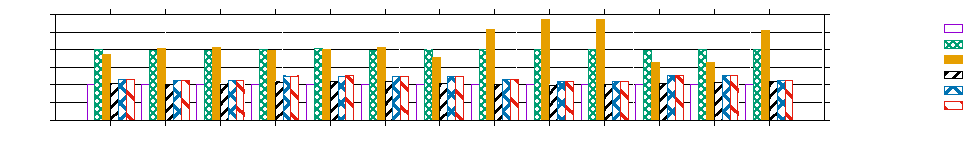
\includegraphics{norm-all_scalar}}%
    \gplfronttext
  \end{picture}%
\endgroup
